\begin{center}\begin{minipage}{\linewidth}
\centering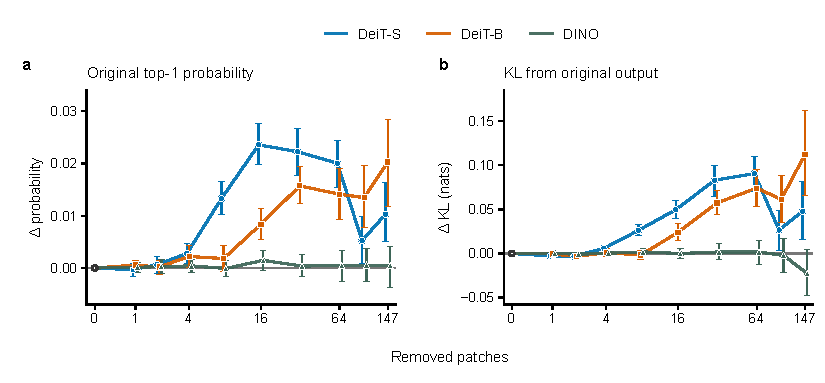
\includegraphics[width=\linewidth]{../../research/v13/endpoints/deletion_curves.pdf}
\captionof{figure}{C3 minus the zero-high-norm control at each original ImageNet-S deletion budget. The probability panel measures least-important-first minus most-important-first target probability. The KL panel reverses the subtraction to express divergence in the same direction. Horizontal positions use a log scale in one plus the number of removed patches, with model-specific offsets for visibility. Intervals are pointwise 95\% paired image-bootstrap intervals over 2,000 images per model. The integrated advantage can coexist with a reversal at a small budget.}
\end{minipage}\end{center}
